%%%%%%%%%%%%%%%%%%%%%%%%%%%%%%%%%%%%%%%%%%%%%%%%%%%%%%%%%%%%%%%%%%%%%%%%%%%%%%%%
%%%%%%%%%%%%%%%%%%   Vorlage für eine Abschlussarbeit   %%%%%%%%%%%%%%%%%%%%%%%%
%%%%%%%%%%%%%%%%%%%%%%%%%%%%%%%%%%%%%%%%%%%%%%%%%%%%%%%%%%%%%%%%%%%%%%%%%%%%%%%%

% Erstellt von Maximilian Nöthe, <maximilian.noethe@tu-dortmund.de>
% ausgelegt für lualatex und Biblatex mit biber

% Kompilieren mit
% latexmk --lualatex --output-directory=build thesis.tex
% oder einfach mit:
% make

\documentclass[
  tucolor,       % remove for less green,
  BCOR=12mm,     % 12mm binding corrections, adjust to fit your binding
  parskip=half,  % new paragraphs start with half line vertical space
  open=any,      % chapters start on both odd and even pages
  cleardoublepage=plain,  % no header/footer on blank pages
]{tudothesis}


% Warning, if another latex run is needed
\usepackage[aux]{rerunfilecheck}

% just list chapters and sections in the toc, not subsections or smaller
\setcounter{tocdepth}{1}

%------------------------------------------------------------------------------
%------------------------------ Fonts, Unicode, Language ----------------------
%------------------------------------------------------------------------------
\usepackage{fontspec}
\defaultfontfeatures{Ligatures=TeX}  % -- becomes en-dash etc.

% german language
\usepackage{polyglossia}
\setdefaultlanguage{german}

% for english abstract and english titles in the toc
\setotherlanguages{english}

% intelligent quotation marks, language and nesting sensitive
\usepackage[autostyle]{csquotes}

% microtypographical features, makes the text look nicer on the small scale
\usepackage{microtype}

%------------------------------------------------------------------------------
%------------------------ Math Packages and settings --------------------------
%------------------------------------------------------------------------------

\usepackage{amsmath}
\usepackage{amssymb}
\usepackage{mathtools}

% Enable Unicode-Math and follow the ISO-Standards for typesetting math
\usepackage[
  math-style=ISO,
  bold-style=ISO,
  sans-style=italic,
  nabla=upright,
  partial=upright,
]{unicode-math}
\setmathfont{Latin Modern Math}

% nice, small fracs for the text with \sfrac{}{}
\usepackage{xfrac}


%------------------------------------------------------------------------------
%---------------------------- Numbers and Units -------------------------------
%------------------------------------------------------------------------------

\usepackage[
  locale=DE,
  separate-uncertainty=true,
  per-mode=symbol-or-fraction,
]{siunitx}
\sisetup{math-micro=\text{µ},text-micro=µ}

%------------------------------------------------------------------------------
%-------------------------------- tables  -------------------------------------
%------------------------------------------------------------------------------

\usepackage{booktabs}       % \toprule, \midrule, \bottomrule, etc

%------------------------------------------------------------------------------
%-------------------------------- graphics -------------------------------------
%------------------------------------------------------------------------------

\usepackage{graphicx}
\usepackage{grffile}
\usepackage{tikz}
\usepackage{circuitikz}
\usepackage{tikz-feynman}
\usepackage{subcaption}

% allow figures to be placed in the running text by default:
\usepackage{scrhack}
\usepackage{float}
\floatplacement{figure}{htbp}
\floatplacement{table}{htbp}

% keep figures and tables in the section
\usepackage[section, below]{placeins}


%------------------------------------------------------------------------------
%---------------------- customize list environments ---------------------------
%------------------------------------------------------------------------------

\usepackage{enumitem}

%------------------------------------------------------------------------------
%------------------------------ Bibliographie ---------------------------------
%------------------------------------------------------------------------------

\usepackage[
  backend=biber,   % use modern biber backend
  autolang=hyphen, % load hyphenation rules for if language of bibentry is not
                   % german, has to be loaded with \setotherlanguages
                   % in the references.bib use langid={en} for english sources
]{biblatex}
\addbibresource{references.bib}  % the bib file to use
\DefineBibliographyStrings{german}{andothers = {{et\,al\adddot}}}  % replace u.a. with et al.


% Last packages, do not change order or insert new packages after these ones
\usepackage[pdfusetitle, unicode, linkbordercolor=tugreen]{hyperref}
\usepackage{bookmark}
\usepackage[shortcuts]{extdash}

%------------------------------------------------------------------------------
%-------------------------    Angaben zur Arbeit   ----------------------------
%------------------------------------------------------------------------------

\author{Nils Breer}
\title{Alignment studies for the LHCb SciFi Detector}
\date{2022}
\birthplace{Unna}
\chair{Lehrstuhl für Experimentelle Physik IV}
\division{Fakultät Physik}
\thesisclass{Master of Science}
\submissiondate{May 4th 2022}
\firstcorrector{Prof.~Dr.~Albrecht}
\secondcorrector{Prof.~Dr.~Weingarten}

% tu logo on top of the titlepage
\titlehead{
\includegraphics[height=1.5cm]{logos/tu-logo.pdf}}

\begin{document}
\frontmatter
\maketitle

% Gutachterseite
\makecorrectorpage

% hier beginnt der Vorspann, nummeriert in römischen Zahlen
\chapter*{Abstract}
\label{sec:abstract}

% general analysis of the scifi detector regarding alignment
% what i have done and how alignment in general has worked out
% difficulties?

% In dieser Bachelorarbeit wird ein Algorithmus zur Rekonstruktion
% von Λ-Baryonen implementiert, welcher auf bereits bestehenden
% Algorithmen zur Rekonstruktion von Kaonen aufbaut und zur Verbesserung
% von Strange-Tagging beiträgt.
% Strange-Tagging ist eine Form des Flavortaggings, welche darauf
% ausgelegt ist, Hadronen mit Strange-Quarks zu identifizieren.
% Vor allem f\"ur neutral geladene Hadronen, welche mindestens ein
% Strange-Quark als Parton tragen ist es interessant
% herauszufinden in welchen Prozessen diese entstehen.
% Au\ss erdem kann das Strange-Tagging dabei helfen, neue Erkenntnisse
% \"uber das CKM-Matrix Element $|\symup{V}_{ts}|$ zu erzielen.
% Dafür werden verschiedene Objekte herangezogen, welche zwischen
% Strange-Quark-Jets und Up-Quark-Jets beziehungsweise Down-Quark-Jets
% diskriminieren.
% Es ergibt sich, dass die Objekte $X_{\symup{\Lambda}}$ und
% $\symup{\Delta R}$ gut zwischen Strange-Jets von Down- und Up-Jets
% diskriminieren doch die Masse des $\symup{\Lambda}$-Baryons daf\"ur
% nicht geeignet ist.

\tableofcontents

\mainmatter
% Hier beginnt der Inhalt mit Seite 1 in arabischen Ziffern
\chapter{Introduction}
\label{sec:einleitung}

At the beginning of the $20^{\text{th}}$ century many physicists started research on
elementary particles and the interactions associated with them. The combined
knowledge lead to the construction of one of the most precisely tested theories: the Standard Model (SM) of particle physics.
Flavour anomalies show strong tensions with the Standard Model and also the recent publication on the W-boson mass measurement is challenging the accuracy of the Standard Model\cite{wmass}.
No single measurement or anomaly on its own is enough to be in a total disagreement with the SM, but combined they provide hints that the SM is not the final theory.
The SM describes every fundamental force except for gravity. There are still open questions such the baryon asymmetry of the universe requiring a, by several orders of magnitude, larger charge-parity (CP) violation than the SM predicted.
To tackle these problems, high energy experiments such as the Large Hadron Collider beauty (LHCb) experiment located at the Large Hadron Collider (LHC) at CERN were built for this exact reason.
The LHCb experiment was designed to study beauty and charm quarks with focus on measuring CP-violation and searching for New Physics in rare decays.
To detect these phenomena, the threshold for statistical uncertainties has to
be lowered and the amount of data collected needs to be increased. The LHCb upgrade described in section \ref{sec:upgradeLHCb} allows us to have a five times higher instantaneous luminosity of $\SI{2e33}{\invfb}$ with the expected detector readout rate of $\SI{40}{\mega\hertz}$.
To realize these hardware and software challenges, the front-end electronics, tracking systems and the trigger system needed upgrades.
The tracking system has been replaced with a single tracker based on scintillating fibres that is currently commissioned. The physics performance is highly dependent on how well the detector is aligned, since poor alignment leads to systematic biases which can have a negative impact on sensitive asymmetry measurements. It can also lead to worse mass resolution. Therefore it is crucial that the SciFi detector is well aligned.
To operate the upgraded LHCb at its full potential, it is of great importance that all detector components are brought into an alignment level so that the impact on physical observables is insignificant.
\\
\\
The Alignment theory will be described in chapter \ref{sec:alignTheory}. In chapter \ref{sec:story} different sets of constraints, degrees of freedom
and alignable objects called \textit{configuration} will be tested first in order
to study how different configurations influence the alignment. Afterwards several
tests will be performed to analyse the behavior of a misaligned detector and check
if the chosen configuration converges towards an aligned state.
The deviations from a centered state after the alignment are needed for other trigger stages to be known in the reconstruction.
The LHC will not run permanently at maximum luminosity therefore tests are performed to analyse alignment of different luminosity samples. Especially while the LHC restarts it will run at a lower luminosity.
During the alignment studies a bias inside the Scintillating Fibre hit clustering algorithms was discovered which had an impact on the alignment. The exact changes will be discussed in the final section of chapter \ref{sec:story}.

% finished

\chapter{The Large Hadron Collider\cite{lhcInfo}}
\label{sec:lhcb}

The Large Hadron Collider (LHC) is the most powerfull particle-accelerator on planet earth. With a circumference of $26,7\si{\kilo\metre}$ it is also the longest ring accelerator and it lies between $45\si{\metre}$ and $170\si{\metre}$ below the surface near Geneva in Swizerland. The tunnel was constructed for the LEP experiment between 1984 and 1989 and is operated by the European Organization for Nuclear Research (CERN). The LHC can produce centre of mass energies of $\sqrt{s} = \SI{13}{\tera\electronvolt}$ in proton-proton collisions during Run 2. After the upgrade the LHC will collide particles with the centre of mass energy $\sqrt{s} = \SI{13}{\tera\electronvolt}$.
An image of the accelerators and the experiments is shown in fig. \ref{fig:CERN}\cite{facilityCERN}.

\begin{figure}
  \centering
  \includegraphics[width=0.5\textwidth]{plots/LHC_facility.ppm}
  \caption{an overview of the LHC facilities.}
  \label{fig:CERN}
\end{figure}

By ionizing hydrogen gas, protonsare created and accelerated to $\SI{50}{\mega\electronvolt}$ by the linear accelerator (LINAC 2). Afterwards the beam is injected into the Proton Syncrotron and the Super Proton Synchrotron to a maximum of $\SI{450}{\giga\electronvolt}$ before the beam is brought into the LHC.
The beam containts several bunches with around $\num{1.15e11}$ and a bunch spacing of $\SI{25}{\nano\seconds}$, which is a collision rate of $\SI{40}{\mega\hertz}$.
The LHC houses four major experiments. ATLAS and CMS are classified as general purpose detectors with a detection range of close to $4\pi$. The interaction in these detectors is located in the very center so that tracks going in every direction can possibly be found. Searches for the Higgs Boson is just one of many physics aspects these detectors are build for.
The other two Experiments located at the LHC are ALICE and LHCb.
The ALICE experiment main studies the quark gluon plasma during the runs with lead ion collisions instead of protons.
In this thesis the Scintillating Fibre Tracker (SciFi Tracker) located at the LHCb will be focused at and discussed on the following chapters.

\section{The LHCb Experiment\cite{lhcbInfo}}

\begin{figure}
  \centering
  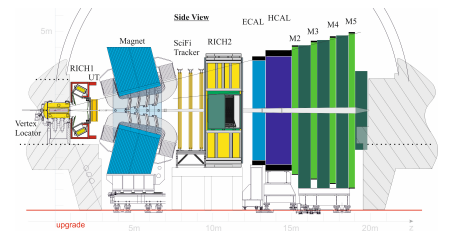
\includegraphics[width=0.5\textwidth]{plots/LHCb_facility.png}
  \caption{a sideview of the LHCb experiment.}
  \label{fig:LHCb}
\end{figure}

The LHCb experiment is a forward spectrometer covering $2 \less \eta \less 5$ in the pseudorapidity range. This experiments main physics goal is beauty quark physics and for high energies, b- and $\bar{b}$-hadrons are heavily produced in a tight forward direction\footnote{They are also produced in a tight backward direction but the experiment is only build for the forward cone.}. A sideview of the LHCb is shown in figure \ref{fig:LHCb}.
The LHCb consists of several smaller detector components namely the Vertex Locator (VELO) right on the intercation point, two Ring Imaging Cherenkov counter (RICH 1 and RICH 2), in front of the spectrometers lies the Trigger Tracker and behind them the SciFi Tracker which is the important part of this thesis. Further back a Scinitllator Pad Detector (SPD) and a Preshower (PS) are mounted followed by the electromagnetic calorimeter and the hadronic calorimeter. In the very back, several muon chambers are mounted for every track that is yet to be determined.

\section{the Scintillating Fibre Tracker\cite{scifiInfo}}
\label{sec:scifi}


% \begin{enumerate}
%   \item layout
%   \item how does it work?
%   \item what else?
% \end{enumerate}

\chapter{Alignment}
\label{sec:alignment}
martinelli pdf! use some of that information
-> alignment is a minimizing problem (chi2) thats why i looked at chi2 plots

-> global translation and sheering motion don't change chi2 values because residuals are unchanged.

-> weak modes: presence of weak modes affect the convergence (poor, takes many iterations), bias in track parameters.

-> most visible weak modes is the "curvature bias" (sophie has mentioned it sometime. must be on one of my sheets)
also look at twiki!
\section{what is alignment used for?}
short answers:
% \begin{enumerate}
%   \item yielding the best possible reconstruction efficiency
%   \item getting a good feeling for particle masses
%   \item momentum resolution of the detector improved
% \end{enumerate}

for these 3 bullet points i need a subsection explaining it!

\section{when does alignment happen?}
at which point during a run will alignment come into play?

\section{Alignment Methods}

\subsection{using tracks fitted with kalman}
talk pdf. quelle herausfinden!
\subsection{'global' alignment with collision data}
wouter pdf. quelle herausfinden!

\section{Alignment goals}
source for now: DPG2021 pdf exact source will be included!
% \begin{enumerate}
%   \item find the best possible configuration of alignables, degrees of freedom, constraints
%   \item check for weak modes (how? chi2, small eigenvalues)
%   \item null tests as good as possible
%   \item misalignment tests to check alignment
% \end{enumerate}

all of the above is just theory. Now, the story i want to tell starts.

%\chapter{Methodik des Strangetaggings}
% Das Strange-Tagging befasst sich damit, Hadronen mit Strange-Quarks
% zu identifizieren.
%
% Analog zum b-Tagging, bei welchem zum Beispiel Sto\ss parameter,
% Flugstrecke, und Zerfallsvertizes verwendet werden um Ausk\"unfte \"uber
% in den Hadronen enthaltene bottom-Quarks zu erhalten,
% kann beim Strange-Tagging, welches hier f\"ur das ungeladene
% $\symup{\Lambda}$-Baryon durchgef\"uhrt wurde, die Informationen von $\symup{\Delta R}$,
% $\symup{p_{T}(\Lambda)} / \symup{p_{T}(\text{Jet})}$ und eventuell der
% origins der Strange-Quarks als Auskunft \"uber Strange-Quarks
% verwendet werden.
%
% In diesem Fall werden $\symup{\Lambda}$-Baryonen mit dem gr\"o\ss ten
% Verzweigungsverhältnis mit zwei Tochterteilchen rekonstruiert.
% Mit den obigen Diskriminanten k\"onnen Aussagen \"uber die Signaleffizienz
% getroffen werden.

\chapter{Results (change title later)}
\label{sec:ergebnisse}

% Die simulierten Samples wurden mit dem Ereignisgenerator
% MADGRAPH\_MC@NLO in f\"uhrender Ordnung von
% $\symup{\alpha}_{S}$ bei einer Schwerpunktsenergie von
% $\sqrt{s} = \SI{13}{\tera\electronvolt}$ generiert.
% Die erzeugten Prozesse sind $pp \rightarrow s\bar{s}$,
% $pp \rightarrow d\bar{d}$ and $pp \rightarrow u\bar{u}$.
% Es wurden jeweils $\num{1000000}$ Ereignisse pro Prozess erzeugt.
% MADGRAPH ist das Standardwerkzeug f\"ur die Erzeugung von Matrixelementen in der Hochenergiephysik.
% Die FEYNMAN-Graphen der Prozesse sind in den Abbildungen
% \ref{fig:feyn1}, \ref{fig:feyn2} und \ref{fig:feyn3} referenziert.
%
% %FEYNMAN-Diagramm f\"ur die Erzeugung des ersten Datensatzes.
\begin{figure}[H]
\centering
\begin{subfigure}{0.3\textwidth}
\feynmandiagram [horizontal=a to b]{
i1 --[gluon, edge label=\(g\)] a --[gluon, edge label=\(g\)] i2,
a --[gluon, edge label=\(g\)] b,
f1 --[fermion, edge label=\(\bar{s}\)] b --[fermion, edge label=\(s\)] f2,
};
\caption{\label{fig:feyn1}}
\end{subfigure}
\begin{subfigure}{0.3\textwidth}
\feynmandiagram [horizontal=a to b]{
i1 --[gluon, edge label=\(g\)] a --[gluon, edge label=\(g\)] i2,
a --[gluon, edge label=\(g\)] b,
f1 --[fermion, edge label=\(\bar{d}\)] b --[fermion, edge label=\(d\)] f2,
};
\caption{\label{fig:feyn2}}
\end{subfigure}
\begin{subfigure}{0.3\textwidth}
\feynmandiagram [horizontal=a to b]{
i1 --[gluon, edge label=\(g\)] a --[gluon, edge label=\(g\)] i2,
a --[gluon, edge label=\(g\)] b,
f1 --[fermion, edge label=\(\bar{u}\)] b --[fermion, edge label=\(u\)] f2,
};
\caption{\label{fig:feyn3}}
\end{subfigure}
\caption{FEYNMAN-Diagramme f\"ur die Erzeugung der Datens\"atze.}
\label{fig:allFeyn}
\end{figure}


% PYTHIA ist ein Werkzeug, welches verwendet wird, um Kollisionen
% im Hochenergiebereich zu erzeugen. Au\ss erdem wird es benutzt um
% verschiedene physikalische Modelle hin zu komplexen Vielteilchen
% Endzust\"anden zu generieren.
% PYTHIA wird meist als \textit{Showerprogramm} verwendet und
% verf\"ugt \"uber Bibliotheken zu Anfangs- bzw. Endzustands
% Partonshowern, Teilchenzerf\"allen und vielem mehr.
%
% \subsection{DELPHES \cite{delph}}
% DELPHES Version 3.4.1 ist ein Simulationsprogramm für radialsymmetrische
% Teilchendetektoren. Hier wird ein Detektor,
% welcher dem CMS-Detektor
% \"ahnelt, verwendet als Beispiel f\"ur einen Multifunktionsdetektor des LHC
% \cite{jerdmannTagger}.
% Es simuliert einen Spurdetektor(Tracker)
% im Inneren eines Magnetfeldes, ein elektromagnetisches(ECAL) und
% ein hadronisches Kalorimeter(HCAL) und außerdem einen Myon-Detektor.
% Es können so physikalische Objekte durch die simulierten
% Detektorantworten rekonstruiert werden. Dafür stehen
% Kalorimetereinträge, Informationen zu Isolationskriterien für
% Elektronen, Tau-Leptonen, sowie Jets und Informationen zur
% fehlenden Energie zur Verfügung. Zur Funktionsweise der einzelnen
% Detektoren, im Spurdetektor werden Teilchenpropagationen betrachtet.
% Dafür wird zwischen geladenen und ungeladenen Teilchen unterschieden.
% Ungeladene Teilchen folgen einer linearen Trajektorie, wohingegen
% geladene Teilchen einer gekrümmten Bahn, abhängig vom Magnetfeld
% folgen. Außerhalb des Trackers startende Teilchenspuren
% werden ignoriert. Für geladene Teilchen kann der Benutzer
% eine Rekonstruktionswahrscheinlichkeit einstellen, mit
% welcher ein Teilchen als Spur im Tracker rekonstruiert
% wird. Die Winkelauflösung sei dabei exakt und der
% Transversalimpuls gemäß einer Gaußkurve verschmiert. Die
% Kalorimeter verschmieren die Energieanteile $f_{\text{ECAL}}$ und $f_{\text{HCAL}}$
% unkorreliert voneinander.
%
% Hinsichtlich der Kalorimeter ist das ECAL für die Energiebestimmung von
% Elektronen und Photonen zuständig und das HCAL für (un-)geladene Hadronen.
% Dies gilt nur für "langlebige" Hadronen. Hierzu zählen $\symup{\Lambda}$-Baryonen und
% Kaonen. Obwohl sie nur eine endliche Lebensdauer haben, gelten sie als stabil.
% Da sie einen nicht zu vernachläßigbaren Anteil ihrer Energie auch im
% ECAL deponieren würden, werden ihre Energiedepositionsanteile zu
% $f_{ECAL} = 0.3$ und $f_{HCAL} = 0.7$ definiert.
% Elektronen und Photonen deponieren ihre gesamte Energie im
% elektromagnetischen Kalorimeter.
%
% In der Objektrekonstruktion werden diverse Annahmen bzgl. der
% Teilchenarten getroffen. Zu den geladenen Leptonen zählen nur
% Elektronen und Myonen, da die Tau-Leptonen zu schnell zerfallen.
% Photonen werden so rekonstruiert, dass Elektronen und Photonen ohne Spur als
% Photon gewertet werden.
% Außerdem kann ein Teilchen isoliert sein. Das ist dann der Fall, wenn sein
% Abstand zu anderen Teilchen kleiner ist als ein definierter Abstand L.
% Ein sehr wichtiger Teil der Objektrekonstruktion ist die der Jets, da diese die
% häufigsten Endzustände bilden.
% DELPHES bietet drei große Jetklassen, welche sich in ihrem Input unterscheiden.
% Zum einen die \textit{Generated Jets}, welche aus langlebigen Teilchen nach
% den Parton-Showern und Hadronisierungsprozessen entstehen. Hierbei werden
% keine Detektorsimulations- bzw. Rekonstruktionsinformationen beachtet.
% Zum Zweiten die \textit{Calorimeter Jets}, welche Kalorimetereinträge als
% Eingabe erhalten und zum Dritten die \textit{particle flow jets}, welche das
% Resultat von Zusammenschlüssen von particle-flow Spuren sind.
% Abschließend werden Informationen über fehlende Transversalenergie
% $\symup{\vec{E}_{T}^{\text{miss}}}$ zurate gezogen, um Aussagen über Teilchen wie die
% Neutrinos zu treffen.
% Dabei ist die fehlende Transversalenergie als
% \begin{equation}
%   \symup{\vec{E}_{T}^{\text{miss}}} = -\sum_{i} \vec{p}_{T}(i)
% \end{equation}
% definiert.


% Das Verzweigungsverh\"altnis des dominanten Zerfalls des Kaons
% wird zuerst bestimmt, um einen Konsistenztest mit den Ergebnissen des
% PDG(particle data group) anzufertigen.
% Im Anschluss wird auch das Verzweigungsverhältnis des dominanten
% Zerfalls des $\symup{\Lambda}$-Baryons bestimmt.
% Damit kann die Validit\"at des Datensatzes \"uberpr\"uft werden.
%
% Hierzu werden die Truth-Informationen der Teilchen verwendet.
% Beginnend mit den $K_{S}$ wird ein
% TLV\footnote{TLorentzVector: Memberfunktion aus ROOT \cite{rootyboy}}
% angelegt welcher den Transversalimpuls, das $\eta$, das $\phi$ und eine
% Massenhypothese speichert. Zwischen diesem Kandidaten und dem Jet mit
% dem h\"ochsten $p_{T}$ wird ein Abstand $\symup{\Delta R}$ von 0.5 definiert,
% der nicht \"uberschritten werden darf.
% Darauffolgend wird \"uberpr\"uft, ob beide Tochterteilchen
% entgegengesetzt geladene Pionen sind. Nur diese werden gez\"ahlt.
% Am Ende wird der Wert der $\pi^{+} \pi^{-}$ Endzust\"ande gez\"ahlt
% und durch die Gesamtanzahl geteilt, um das Verzweigungsverhältnis
% zu erhalten.
%
% \"Ahnlich wird f\"ur die $\symup{\Lambda}$-Baryonen verfahren. Es wird
% wieder gez\"ahlt wie viele Tochterteilchenpaare aus
% $p \pi^{-}$ bzw. $\pi^{-} p$ bestehen und wie viele Paare
% insgesamt vorhanden sind.
% Der Bruchteil
% \begin{equation}
%   \text{BR} = \frac{\text{Counts}(p \pi^{-} + \pi^{-} p)}{\text{Counts(all)}}
% \end{equation}
% ist das Verzweigungsverhältnis mit der h\"ochsten Wahrscheinlichkeit
% f\"ur den $\symup{\Lambda}$-Zerfall.
% Dies wird f\"ur jedes der drei generierten Samples
% $\symup{pp}\rightarrow\symup{s\bar{s}}$,
% $\symup{pp}\rightarrow\symup{d\bar{d}}$
% und $\symup{pp}\rightarrow\symup{u\bar{u}}$ durchgef\"uhrt.
%
% Die dazugeh\"origen Messwerte befinden sich in Tabelle \ref{tab:truthBR}.
% \begin{table}
% \centering
% \caption{Zerfallsbreiten f\"ur das $K_S$ und das  $\symup{\Lambda}_0$-Baryon \cite{kaonPDG}, \cite{lambdaPDG}.}
% \label{tab:truthBR}
% \begin{tabular}{c|c c|c c}
% \toprule
% $\text{Sample}$
% & \multicolumn{2}{c}{$\Lambda \rightarrow p\pi^{-}$}
% & \multicolumn{2}{c}{$K_S \rightarrow \pi^{+}\pi^{-}$} \\
% $\text{Prozess}$ & $\text{BR}$ & $\text{BR(PDG)}$
% & $\text{BR}$ & $\text{BR(PDG)}$ \\
% \midrule
% $\text{pp} \rightarrow s\bar{s}$ & $\SI{65.26}{\percent}$ & $\SI{63.90(05)}{\percent}$ & $\SI{70.95}{\percent}$ & $\SI{69.20(05)}{\percent}$ \\
% $\text{pp} \rightarrow d\bar{d}$ & $\SI{64.90}{\percent}$ & $\SI{63.90(05)}{\percent}$ & $\SI{71.11}{\percent}$ & $\SI{69.20(05)}{\percent}$ \\
% $\text{pp} \rightarrow u\bar{u}$ & $\SI{65.04}{\percent}$ & $\SI{63.90(05)}{\percent}$ & $\SI{70.96}{\percent}$ & $\SI{69.20(05)}{\percent}$ \\
% \bottomrule
% \end{tabular}
% \end{table}
%
% Die berechneten Verzweigungsverhältnisse des $\symup{\Lambda}$-Zerfalls
% weichen alle jeweils um $\left(\num{1} - \num{2}\right)\si{\percent}$
% von den Werten im PDG ab. Dies kann an der relativ kleinen Statistik
% liegen. Es wurden in jedem Sample nur eine Millionen Ereignisse
% generiert. Demnach ist diese Abweichung plausibel, sodass
% eine gute Konsistenz mit dem PDG vorliegt.
% Die berechneten Verzeigungsverh\"altnisse des dominanten $\symup{K}_{S}$-Zerfalls weichen auch um wenige Prozent von den PDG-Werten ab.
% Dies liegt wahrscheinlich ebenfalls an der kleinen Statistik und ist dadurch erkl\"arbar.
% Zusammenfassend bedeutet das, dass die Samples valide sind und eine weitere Analyse keine grundlegend falschen Ergebnisse liefern sollte.

\newpage

% Einleitend in die Rekonstruktion des $\symup{\Lambda}$-Baryons ist der dominante
% Zerfall in Abbildung \ref{fig:ldecay} dargestellt.
%
% \begin{figure}
\centering
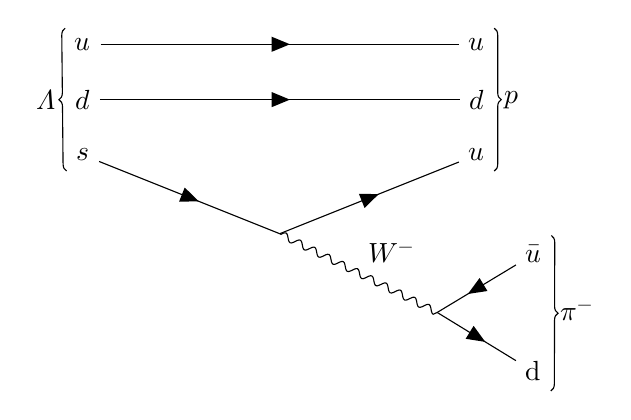
\begin{tikzpicture}
\begin{feynman}
\vertex (u) {\(u\)};
\vertex[right=5cm of u] (uu) {\(u\)};
\vertex[below=2em of u] (d) {\(d\)};
\vertex[right=5cm of d] (dd) {\(d\)};
\vertex[below=2em of d] (s) {\(s\)};
\vertex[right=5cm of s] (uuu) {\(u\)};
\vertex[below right=1cm and 2.5cm of s] (v1);
\vertex[below right=1cm and 2cm of v1] (v2);
\vertex[above right=0.5cm and 1cm of v2] (ubar) {$\bar{u}$};
\vertex[below right=0.5cm and 1cm of v2] (dnorm) {$\symup{d}$};
\diagram* { {[edges=fermion]
(u) -- (uu),
(d) -- (dd),
(s) -- (v1) -- (uuu),
(ubar) -- (v2) -- (dnorm)},
(v1) -- [boson, edge label=\(W^{-}\)] (v2)
};
\draw [decoration={brace}, decorate] (s.south west) -- (u.north west) node [pos=0.5, left] {\(\Lambda\)};
\draw [decoration={brace}, decorate] (uu.north east) --  (uuu.south east) node [pos=0.5, right] {\(p\)};
\draw [decoration={brace}, decorate] (ubar.north east) --  (dnorm.south east) node [pos=0.5, right] {\(\pi^{-}\)};
\end{feynman}
\end{tikzpicture}
\caption{FEYNMAN Diagramm des dominanten $\symup{\Lambda}$-Baryon Zerfalls.}
\label{fig:ldecay}
\end{figure}

%
% Mein Auswertungsprogramm zur $\symup{\Lambda}$-Rekonstruktion wurde mit dem Hochenergieframework ROOT f\"ur C++ geschrieben, demnach werden viele Methoden aus diesem verwendet.
%
% % charge criteria of track pairs
% Das $\symup{\Lambda}$-Baryon ist ein neutral geladenes Baryon, welches in zwei Tochterteilchen zerf\"allt.
% Demnach m\"ussen diese entgegengesetzt geladen oder beide neutral geladen sein.
%
% Da der Zerfall $\symup{\Lambda} \rightarrow \symup{n}\pi^{0}$ aufgrund von neutral geladenen Spuren des Neutrons und des $\pi^{0}$ nicht von DELPHES simuliert werden kann ist der einzige zu betrachtene Zerfall
% $\symup{\Lambda} \rightarrow \symup{p}\pi^{-}$.
% Demnach werden weiter nur Spurpaare verwendet, welche eine
% multiplizierte Ladung von -1 haben, also unterschiedlich geladen sind.
%
% % reference lambda
% Nun wurde ein \textit{TLV} f\"ur ein $\symup{\Lambda}$-Baryon erstellt. Dieses wird als
% Referenz f\"ur jegliche Vergleiche und Kriterien verwendet.
% Dieser \textit{TLV} enth\"alt Informationen \"uber den Transversalimpuls $\symup{p}_{\symup{T}}$,
% die Pseudorapidit\"at $\eta$, den Azimutalwinkel $\phi$ und eine Massenhypothese.
%
% Im Anschluss werden Kandidaten f\"ur $\symup{\Lambda}$-Baryonen erzeugt.
% Diese bestehen aus zwei Spuren korrespondierend f\"ur zwei Tochterteilchen.
% Erzeugt werden diese wieder mit Hilfe eines \textit{TLorentzVector}
% f\"ur jeweils den ersten und zweiten Eintrag eines Spurpaares.
% In diesen stecken die Hypothesen der Protonenmasse f\"ur Spur 1 und die
% der Pionmasse f\"ur Spur 2.
% Das liegt daran, dass das Proton in den meisten F\"allen mit
% dem h\"oheren Transversalimpuls eingeht \cite{stquelle}.
% Der Kandidat besteht nun aus der Summe der beiden Spuren.
% Dieser weist nun vier Parameter auf. $\symup{p}_{\symup{T}}$, $\eta$, $\phi$ und
% einer Masse, welche aus dem Spurpaar durch Addition beider \textit{TLV} gebildet wird.
% Es werden au\ss erdem nur Kandidaten ausgew\"ahlt, welche einen Abstand
% $\symup{\Delta R}$ zur Jetachse haben, mit $\symup{\Delta R} < \num{0.5}$.
% Dabei ist $\symup{\Delta R} =
% \sqrt{\Delta\phi^{2} + \Delta\eta^{2}}$, $\eta$ ist die
% Pseudorapidit\"at und $\phi$ ist der Azimutalwinkel.
% Der Grund daf\"ur ist ein "geometrisches Matching" des Kandidaten mit
% dem s- oder $\bar{s}$-Jet, weshalb $|\symup{\Delta R}| < \num{0.5}$
% sein muss.
% Zus\"atzlich soll der Transversalimpuls der Kandidaten  gr\"o\ss er als
% $\SI{1}{\giga\electronvolt}$ sein, da daf\"ur die Effizienz des Trackers
% $\SI{95}{\percent}$ ist \cite{jerdmannTagger}.
% Au\ss erdem muss der Transversalimpuls der Jets gr\"o\ss er als
% $\SI{20}{\giga\electronvolt}$ sein, bei einem maximalen
% $\eta(\text{Jet}) = \num{2.5}$.
% Danach werden die PIDs(particle Identification) der beiden Spuren der Kandidaten betrachtet.
% Damit keine $\pi^{+}\pi^{-}$ Endzustände weiterverwendet werden, werden alle
% Spurpaare mit $\text{PDGID}\footnote{particle data group Identification: Jedes
% Teilchen tr\"agt eine individuelle Nummer}(Spur 1) = \pm \num{211}$ und
% $\text{PDGID}(Spur 2) = \mp \num{211}$ verworfen.
% Um zu garantieren, dass keine $\symup{\Lambda}$-Antibaryonen im reduzierten
% Sample verbleiben, werden au\ss erdem die Spurpaare entfernt die
% $\text{PDGID}(\text{Spur} 1) = \text{PDGID}(\text{Antiproton})$ und $\text{PDGID}(\text{Spur} 2) = \text{PDGID}(\pi^{+})$ tragen.

\newpage

%$\symbf{hier\, muss\, einiges\, nochmal\, neu\, geschrieben\, werden...}$\\

% Aus den in Kapitel \ref{sec:ereignissel} genannten Objekten werden
% die ausgewählt, die eine diskriminierende Wirkung zwischen
% den Datensätzen, zeigen könnten.
%
% Vorüberlegungen ergeben, dass zum ersten $X_{\Lambda}$, also
% $\frac{p_{T}(\Lambda)}{p_{T}(\text{Jet})}$ als Diskriminator
% fungieren könnte.
% Bei der Betrachtung der FEYNMAN-Graphen in den Abbildungen
% \ref{fig:feyn1}, \ref{fig:feyn2} und \ref{fig:feyn3} gibt es einen entscheidenden Unterschied.
% In dem Prozess $pp \rightarrow s\bar{s}$ ist es m\"oglich,
% dass die Strange-Quarks nach der Hadronisierung und Parton-Showern
% Bestandteil eines $\symup{\Lambda}$-Baryons sind.
% Das bedeutet, dass sie ihren vollen Transversalimpuls in das
% $\symup{\Lambda}$ tragen.
% Wohingegen $\symup{\Lambda}$, die nach der Hadronisierung aus dem
% Prozess $pp \rightarrow d\bar{d}(u\bar{u})$ enstehen, ein
% Strange-Quark ben\"otigen.
% Dieses kann nur w\"ahrend der Hadronisierung entstehen.
% Bis sich ein $\symup{\Lambda}$-Baryon gebildet hat, kann das Strange-Quark aber
% noch Teile seines Transversalimpulses abgeben, wodurch im Mittel
% der Gesamttransversalimpuls niedriger sein m\"usste als der von den $\symup{\Lambda}$-Baryonen die durch den Prozess $pp \rightarrow s\bar{s}$ initiiert wurden.
%
% Zum Zweiten wurde $\symup{\Delta R}$, welches der Abstand
% zweier Spuren oder eines gesuchten Teilchens und eines Jets in
% der $\eta$ - $\phi$ - Ebene beschreibt, gew\"ahlt.
% Wenn das in Abbildung \ref{fig:feyn1} erzeugte Strange-Quark f\"ur ein
% $\symup{\Lambda}$-Baryon verwendet wird, liegt der Jet weitestgehend in Richtung der
% Hadronisierung, das bedeutet, dass $\symup{\Delta R}$ in den meisten F\"allen kleiner ist, als wenn ein Strange-Quark aus der Hadronisierung Bestandteil eines $\symup{\Lambda}$-Baryons sein w\"urde.
% Wenn die Quarks, welche gem\"a\ss\, Abbildung \ref{fig:feyn2} und \ref{fig:feyn3}
% erzeugt werden, Bestandteile eines $\symup{\Lambda}$-Baryons werden, werden die Abst\"ande zwischen dem gesuchten Teilchen und dem dazugeh\"origen Jet gr\"o\ss er sein. Somit ergibt sich vermutlich auch eine diskriminierende Wirkung. Die \"Uberlegung, die Masse des $\symup{\Lambda}$ zu verwenden, l\"asst sich leicht als Sackgasse
% identifizieren, da die Verteilungsfunktion der Masse f\"ur alle drei Datens\"atze fast exakt \"ubereinander liegen sollten, da die Masse nicht vom Erzeugungszeitpunkt abh\"angen darf. Demnach ist hier keine diskriminierende Wirkung zu erwarten.
%
% In den Abbildungen \ref{fig:deltaR}, \ref{fig:xlambda} und
% \ref{fig:massL} sind die Plots der jeweiligen Diskriminante
% gegen die H\"aufigkeit aufgetragen. In Abbildung
% \ref{fig:deltaR} ist zu erkennen, dass $\symup{\Lambda}$-Baryonen mit Strange-Quark aus dem Prozess
% $pp \rightarrow s\bar{s}$ weniger weit von der Jetachse abweichen als $\symup{\Lambda}$-Baryonen die ein Strange-Quarks nach der Hadronisierung verwenden.
% Dies bekr\"aftigt auch die Hypothese
% aus Kapitel \ref{sec:disk}. In Abbildung \ref{fig:xlambda} ist
% die Verteilung von $X_{\Lambda}$ gegen\"uber
% der H\"aufigkeit dargestellt. Es ist klar
% zu erkennen, dass $\symup{\Lambda}$-Baryonen, welche aus $pp \rightarrow s\bar{s}$ Prozessen initiiert werden
% h\"aufiger h\"ohere Transversalimpulse haben
% (schwarze Kurve), als solche, die auf die anderen beiden Arten entstehen.
%
% \begin{figure}
%   \centering
%   \includegraphics[width=0.8\textwidth]{../../../../../../bscnilsbreer_new/BA_NilsBreer_2019/output/DeltaR_A3.pdf}
%   \caption{Plot f\"ur den Abstand $\symup{\Delta R}$ zwischen dem Jet in f\"uhrender $\symup{p}_{\symup{T}}$ Ordnung und dem Rekonstruierten $\symup{\Lambda}$-Baryon.}
%   \label{fig:deltaR}
% \end{figure}
%
% \begin{figure}
%   \centering
%   \includegraphics[width=0.8\textwidth]{../../../../../../bscnilsbreer_new/BA_NilsBreer_2019/output/XLambda.pdf}
%   \caption{Plot f\"ur das Transversalimpulsverh\"altnis des $\symup{\Lambda}$-Baryons zum Jet-Transversalimpuls.}
%   \label{fig:xlambda}
% \end{figure}
%
% \begin{figure}
%   \centering
%   \includegraphics[width=0.8\textwidth]{../../../../../../bscnilsbreer_new/BA_NilsBreer_2019/output/LInvMass_true_p_pi.pdf}
%   \caption{Invariante $\symup{\Lambda}$-Baryon-Masse $\sqrt{\symup{s}}$ in $\si{\mega\electronvolt}$.}
%   \label{fig:massL}
% \end{figure}
%
% \newpage

% Da ein Algorithmus zur Rekonstruktion von $K_{S}$ bereits zur Verf\"ugung
% stand, wurden f\"ur diese ROC-Kurven im Hinblick auf
% die selben Diskriminanten wie f\"ur die $\symup{\Lambda}$-Baryonen erstellt.
% Das Ziel ist es, diese Ergebnisse als Vergleich bzw. f\"ur einen
% Konsistenztest zu verwenden.
%
% Die erstellten Kurven befinden sich in den Abbildungen
% \ref{fig:kaon_roc_sd} und \ref{fig:kaon_roc_su}.
% Aufgetragen auf der y-Achse ist
% die Sensitivit\"at des Strange-Quark Monte-Carlo-Samples, welche
% der Bruchteil der "true positives" \"uber der Gesamtzahl ist.
% Sie ist ein Ma\ss\, f\"ur die Signaleffizienz (SE). Auf der x-Achse ist
% 1-Spezifizit\"at des Down-Quark Monte-Carlo-Samples aufgetragen. Sie entspricht der Hintergrundeffizienz(BE).
% Die rote Kurve stellt die Linie dar, bei welcher der Algorithmus Zufallswerte liefern w\"urde. Liegt die Kurve dar\"uber, arbeitet der Algorithmus gut. Liegt die Kurve darunter arbeitet er dementsprechend schlechter.
%
% In beiden Abbildungen ist zu erkennen, dass die Variablen $X_{K}$ und
% $\symup{\Delta R}$, wie bei den $\symup{\Lambda}$-Baryonen, ziemlich gut
% diskriminieren und gut f\"ur die Rekonstruktion geeignet sind.
% Es ist auch zu sehen, dass mithilfe der Masse keine Aussage bez\"uglich
% der Signaleffizienz getroffen werden kann.
%
% \begin{figure}
%   \centering
%   \includegraphics[width=0.8\textwidth]{../../../../../../bscnilsbreer_new/BA_NilsBreer_2019/py_output/kaon_ROC_s_d.pdf}
%   \caption{ROC Kurve f\"ur den Vergleich zwischen $\text{s}\bar{\text{s}}$ und $\text{d}\bar{\text{d}}$ Sample f\"ur Kaonen.}
%   \label{fig:kaon_roc_sd}
% \end{figure}
%
% \begin{figure}
%   \centering
%   \includegraphics[width=0.8\textwidth]{../../../../../../bscnilsbreer_new/BA_NilsBreer_2019/py_output/kaon_ROC_s_u.pdf}
%   \caption{ROC Kurve f\"ur den Vergleich zwischen $\text{s}\bar{\text{s}}$ und $\text{u}\bar{\text{u}}$ Sample f\"ur Kaonen.}
%   \label{fig:kaon_roc_su}
% \end{figure}
%
% Um nun etwas \"uber die Aussagekr\"aftigkeit der Diskriminanten
% bez\"uglich des $\symup{\Lambda}$-Baryons zu sagen,
% wurden auch ROC-Kurven, zusehen in
% den Abbildungen \ref{fig:roc_sd} und \ref{fig:roc_su}
% %\cite{roccy1}, \cite{roccy2}
% angefertig, welche die Ergebnisse veranschaulichen und
% G\"ute der Diskriminanten validieren sollen. Dazu wurden die
% Ergebnisse resultierend aus dem Datensatz mit $s\bar{s}$ im
% Endzustand mit jeweils einem der beiden anderen verglichen.
%
% Dargestellt sind die Diskriminanten $X_{\Lambda}$,
% $\symup{\Delta R}$ und $M_{\Lambda}$.
% An der schwarzen Kurve ist zu erkennen, dass sie relativ weit \"uber der
% roten Kurve liegt, $X_{\Lambda}$ also als diskriminierende Variable
% zu gebrauchen ist.
% Es ist auch zu erkennen, dass bei kleiner werdender SE die BE auch kleiner wird, doch in einem st\"arkeren Ma\ss.
%
% Die blaue Kurve von $\symup{\Delta R}$ liegt auch noch \"uber
% der roten Kurve, aber nicht mehr so weit wie die schwarze. $\symup{\Delta R}$
% ist also noch als Diskriminator zu verwenden.
% Die gr\"une Kurve liegt sehr genau auf
% der roten Kurve, weshalb diese Variable nicht als Diskriminante
% zu verwenden ist.
%
% Wie zu erwarten arbeiten $\symup{\Delta R}$ und $X_{\Lambda}$
% gut als Diskriminanten.
%
% \newpage
%
% \begin{figure}
% \centering
% \begin{subfigure}{\textwidth}
%   \centering
%   \includegraphics[width=0.8\textwidth]{../../../../../../bscnilsbreer_new/BA_NilsBreer_2019/py_output/ROC_s_d.pdf}
%   \caption{ROC-Kurve f\"ur $\symup{\Lambda}$-Baryonen zwischen Samples mit $s\bar{s}$ Endzustand und $d\bar{d}$ Endzustand.}
%   \label{fig:roc_sd}
% \end{subfigure}
% \begin{subfigure}{\textwidth}
%   \centering
%   \includegraphics[width=0.8\textwidth]{../../../../../../bscnilsbreer_new/BA_NilsBreer_2019/py_output/ROC_s_u.pdf}
%   \caption{ROC-Kurve f\"ur $\symup{\Lambda}$-Baryonen zwischen Samples mit $s\bar{s}$ Endzustand und $u\bar{u}$ Endzustand.}
%   \label{fig:roc_su}
% \end{subfigure}
% \caption{ROC-Kurven f\"ur $\symup{\Lambda}$-Baryonen.}
% \label{fig:ROCCY}
% \end{figure}

\chapter{Conclusion}


\appendix
% Hier beginnt der Anhang, nummeriert in lateinischen Buchstaben
%\chapter{Ein Anhangskapitel}
Hier könnte ein Anhang stehen, falls Sie z.\,B.\ Code, Konstruktionszeichnungen oder Ähnliches mit in die Arbeit bringen wollen.
Im Normalfall stehen jedoch alle Ihre Resultate im Hauptteil der Bachelorarbeit und ein Anhang ist überflüssig.


\backmatter
\printbibliography
\chapter*{Danksagung}
An dieser Stelle m\"ochte ich mich bei all denen bedanken,
die mir w\"ahrend meiner Bachelorarbeit zur Seite standen und
ich mich immer unterst\"utzt haben.

Zuerst m\"ochte ich ich bei Herrn Professor Dr. Kevin Kr\"oninger
bedanken, durch welchen ich an seinem Lehrstuhl meine Bachelorarbeit
schreiben konnte. Au\ss erdem m\"ochte ich mich bei der Abteilung der
ATLAS Datenanalyse f\"ur die konstruktiven Anregungen bedanken.

Einen gro\ss en Dank spreche ich vor allem meinem Betreuer Dr.
Johannes Erdmann aus, der mich mit voller Unterst\"utzung und
wertvollen Ratschl\"agen und Hilfestellungen durch meine
Bachelorarbeit begleitet hat. Durch ihn habe ich viel
gelernt und bei Fragen konnte er mir stehts weiterhelfen.

Ich m\"ochte mich auch bei Herrn Professor Dr. Bernhard Spaan
f\"ur die Zweitkorrekur meiner Arbeit bedanken.

Mein Dank geb\"urt au\ss erdem Christopher Krause, Jan Lukas
Sp\"ah, Michael Windau, Sebastian L\"utge und Christian Beckmann
f\"ur die fachliche Kompetenz bei Fragen aller Art.

Zuletzt m\"ochte ich meiner Familie und Freunden daf\"ur danken,
dass sie mich w\"ahrend meines gesamten Studiums immer
unterst\"utzt und motiviert haben.

\cleardoublepage
\thispagestyle{empty}
% \section*{Eidesstattliche Versicherung}
% Ich versichere hiermit an Eides statt, dass ich die vorliegende Abschlussarbeit mit dem Titel \enquote{\thetitle} selbstständig und ohne unzulässige fremde Hilfe erbracht habe.
% Ich habe keine anderen als die angegebenen Quellen und Hilfsmittel benutzt, sowie wörtliche und sinngemäße Zitate kenntlich gemacht.
% Die Arbeit hat in gleicher oder ähnlicher Form noch keiner Prüfungsbehörde vorgelegen.
%
% \vspace*{1cm}\noindent
% \begin{center}
%   \begin{tabular}{@{}p{0.4\textwidth}@{\hspace{0.15\textwidth}}p{0.4\textwidth}@{}}
%   \rule{\linewidth}{0.25pt}& \rule{\linewidth}{0.25pt}\\
%   Ort, Datum & Unterschrift
%   \end{tabular}
% \end{center}
%
% \subsection*{Belehrung}
% Wer vorsätzlich gegen eine die Täuschung über Prüfungsleistungen betreffende Regelung einer Hochschulprüfungsordnung verstößt, handelt ordnungswidrig.
% Die Ordnungswidrigkeit kann mit einer Geldbuße von bis zu \SI[round-mode=places, round-precision=2]{50000}{€} geahndet werden.
% Zuständige Verwaltungsbehörde für die Verfolgung und Ahndung von Ordnungswidrigkeiten ist der Kanzler/die Kanzlerin der Technischen Universität Dortmund.
% Im Falle eines mehrfachen oder sonstigen schwerwiegenden Täuschungsversuches kann der Prüfling zudem exmatrikuliert werden \mbox{(\S\,63 Abs. 5 Hochschulgesetz --HG--).}
%
% Die Abgabe einer falschen Versicherung an Eides statt wird mit Freiheitsstrafe bis zu 3 Jahren oder mit Geldstrafe bestraft.
%
% Die Technische Universität Dortmund wird ggf.\ elektronische Vergleichswerkzeuge (wie z.\,B.\ die Software \enquote{turnitin}) zur Überprüfung von Ordnungswidrigkeiten in Prüfungsverfahren nutzen. \\[\baselineskip]
%
% \noindent Die oben stehende Belehrung habe ich zur Kenntnis genommen.\\[1cm]
% \begin{center}
% \begin{tabular}{@{}p{0.4\textwidth}@{\hspace{0.15\textwidth}}p{0.4\textwidth}@{}}
% \rule{\linewidth}{0.25pt}& \rule{\linewidth}{0.25pt}\\
% Ort, Datum & Unterschrift
% \end{tabular}
% \end{center}

\begin{figure}
  \centering
  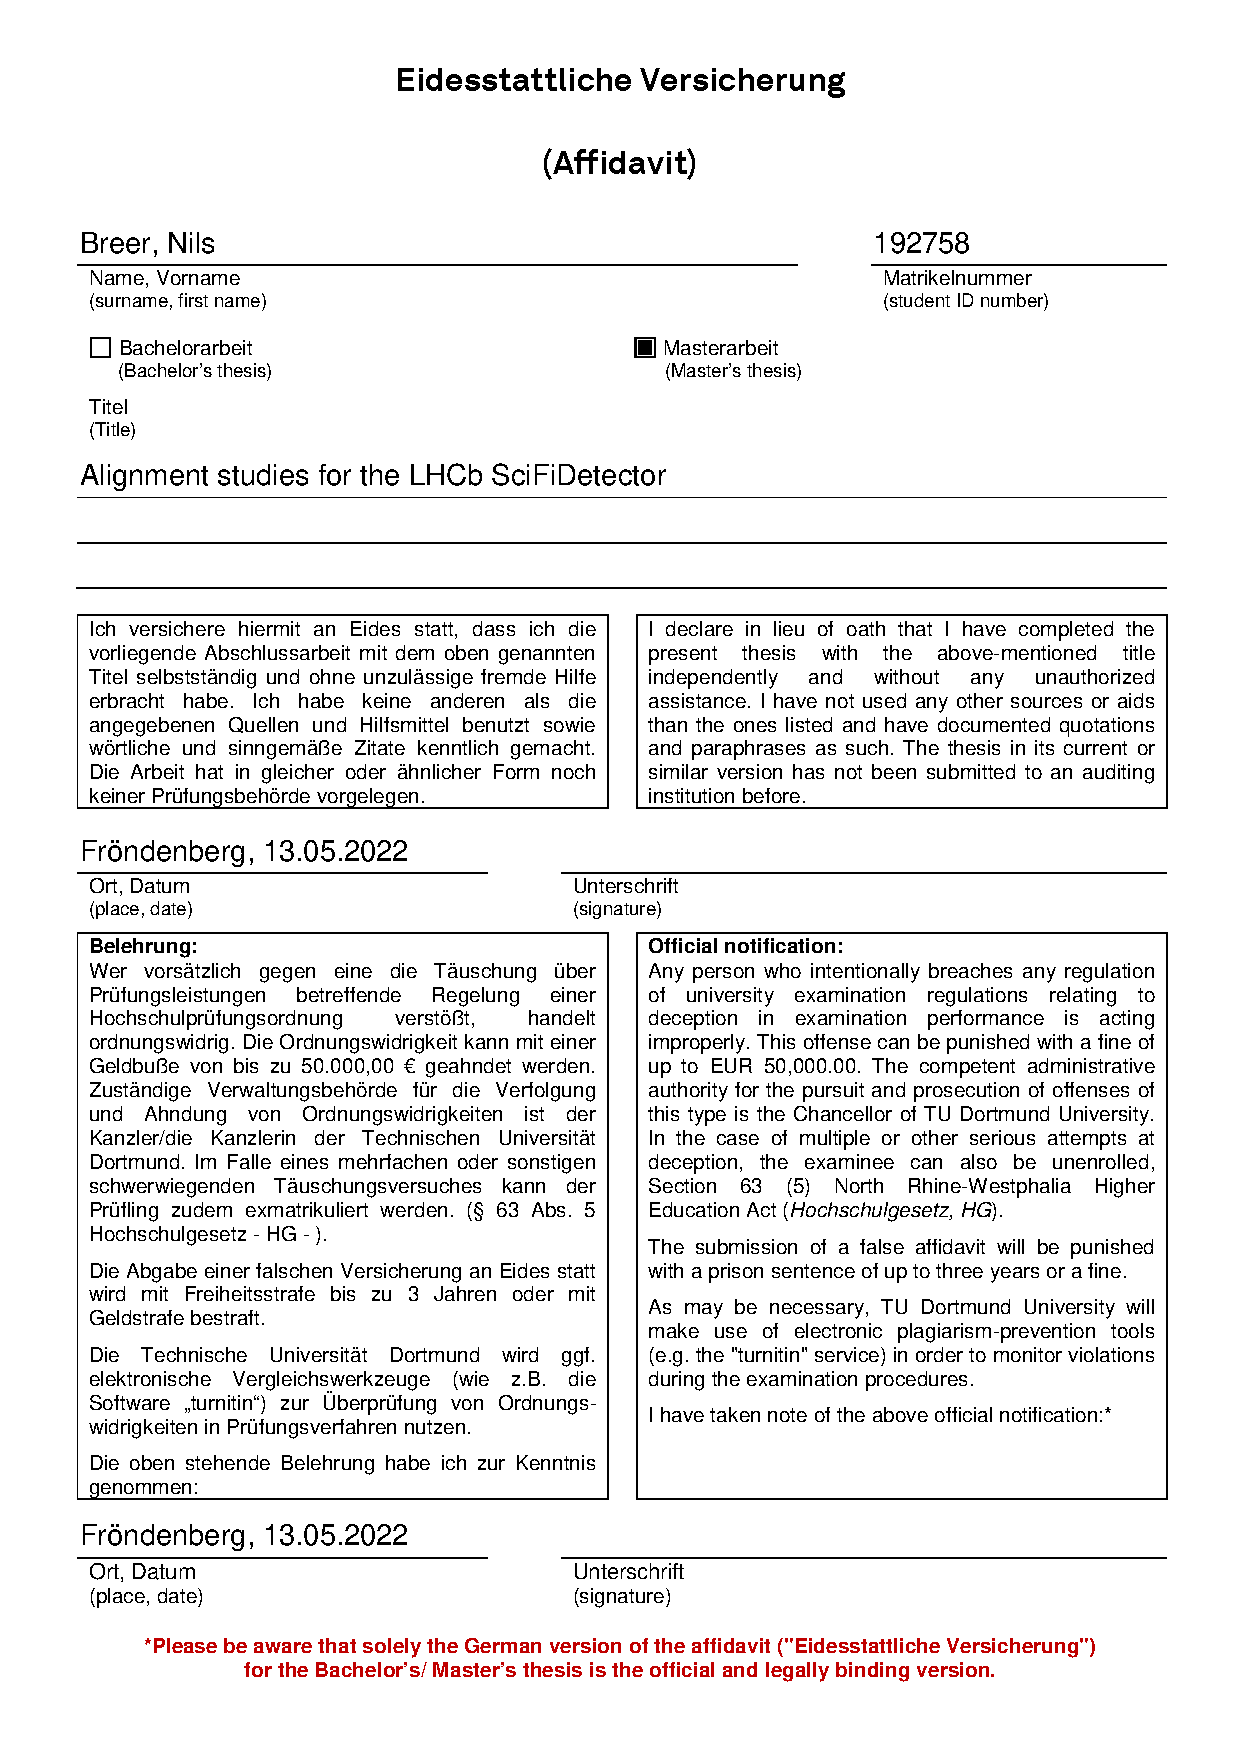
\includegraphics[width=\textwidth]{Eidesstattliche_Versicherung.pdf}
\end{figure}

\end{document}
